\title{T-61.5130 Machine Learning and Neural Networks}
\author{Karhunen, Luttinen}
\date{Exercise 4}

% \usepackage[english]{babel}
% \usepackage[latin1]{inputenc}
% \usepackage{subfigure}
% \usepackage{epsfig}
% \usepackage{amsmath,amssymb}
% \usepackage{psfrag}
% \parindent 0mm
% \textwidth 16cm
% \textheight 23cm
% \oddsidemargin 0cm
% \evensidemargin 0cm
% \topmargin -10mm

\newcommand{\vect}[1]{{\bf{#1}}}
\newcommand{\svect}[1]{\boldsymbol{#1}}
\newcommand{\matr}[1]{\boldsymbol{#1}}


\begin{document}

\maketitle
\thispagestyle{empty}

\begin{enumerate}

\item Construct a MLP network which is able to separate the two
  classes illustrated in Figure \ref{fig:mlp_classify}. Use two neurons both in the input
  and output layer and an arbitrary number of hidden layer
  neurons. The output of the network should be vector $\left[ 1,
    0\right]^T$ if the input vector belongs to class $\mathcal{C}_1$ and  $\left[ 0,
    1\right]^T$ if it belongs to class $\mathcal{C}_2$. Use nonlinear activation
  functions, namely McCulloch-Pitts model, for all the neurons and
  determine their weights by hand without using any specific learning
  algorithm.
  \begin{enumerate}
  \item What is the minimum amount of neurons in the hidden layer
    required for a perfect separation of the classes?
  \item What is the maximum amount of neurons in the hidden layer?
  %\item Is one layer sufficient to classify any two separable classes?
  \end{enumerate}

  \begin{figure}[hbp]
    \centering
    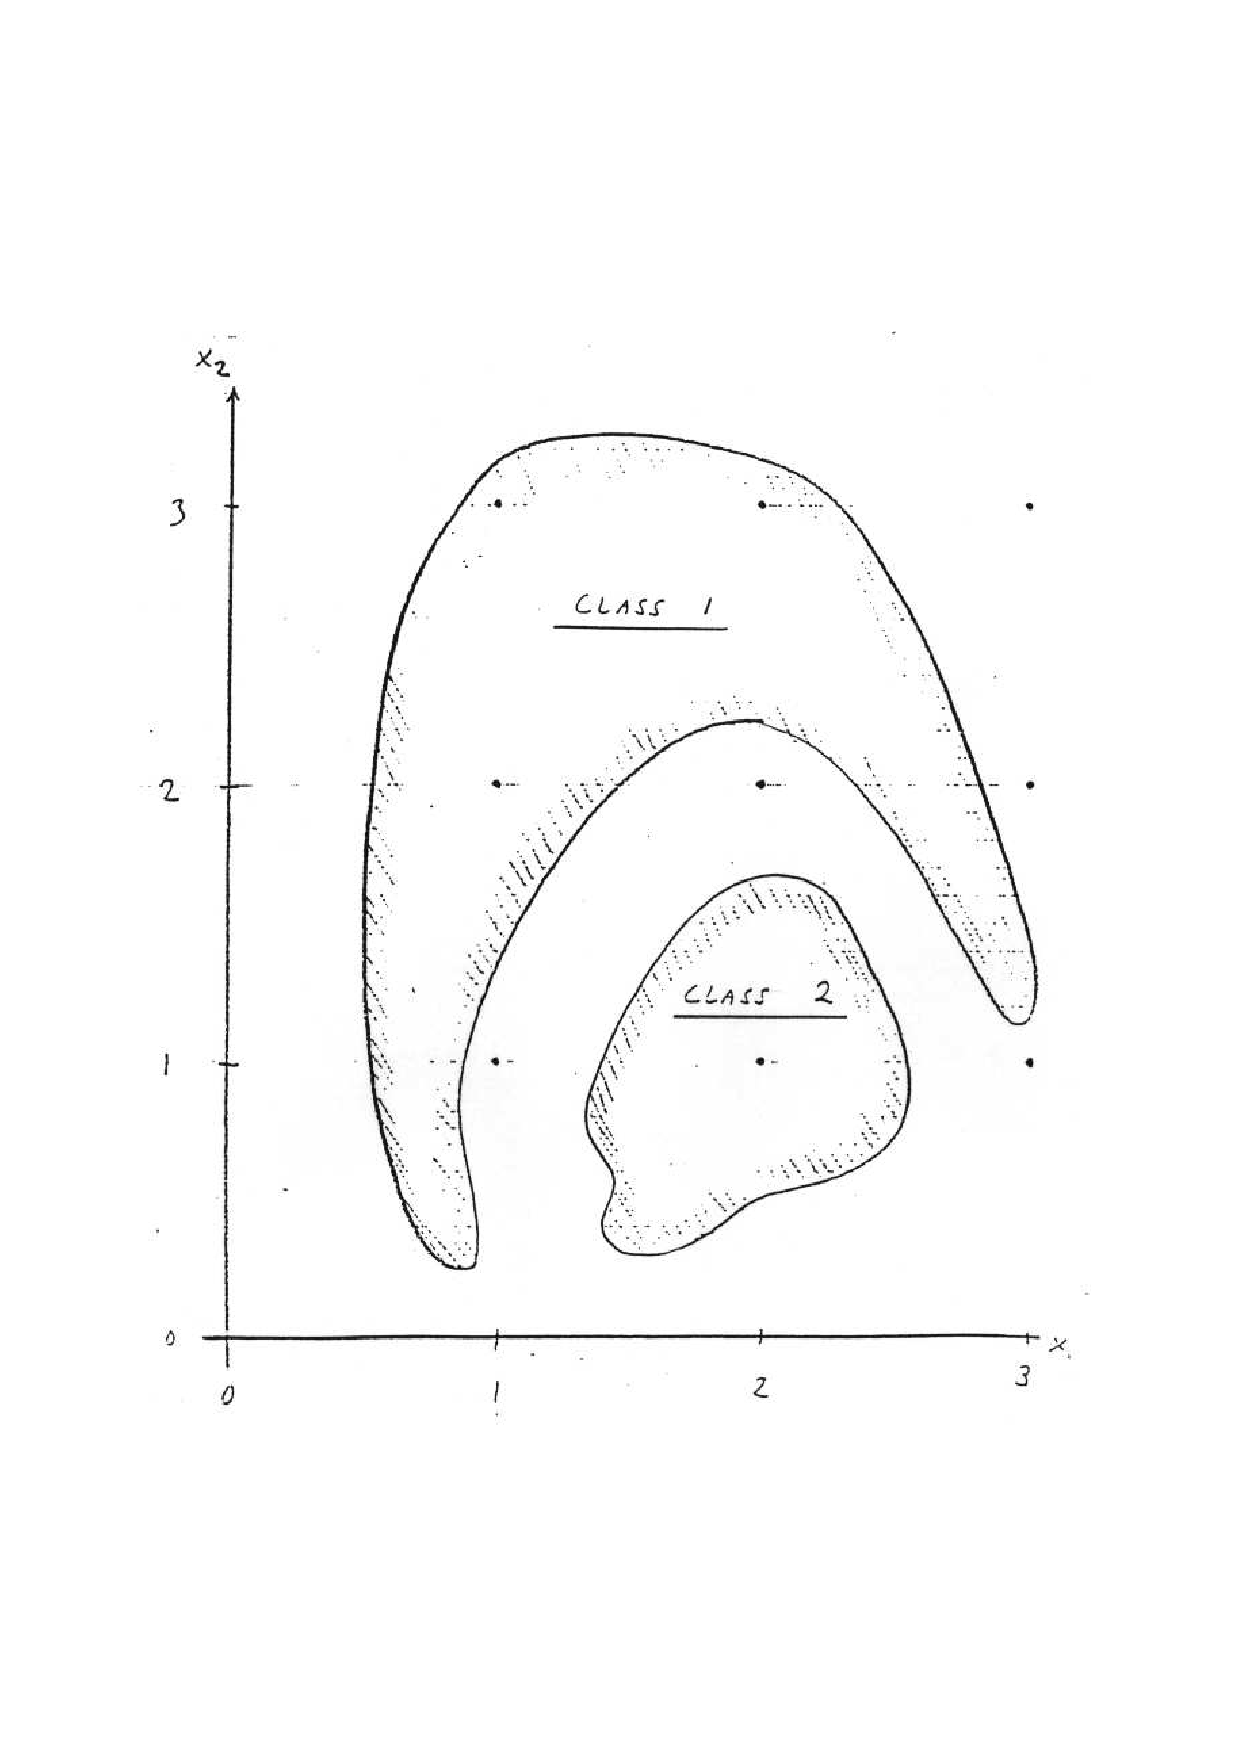
\includegraphics[width=7cm]{mlp_classification}
    \caption{Classes $\mathcal{C}_1$ and $\mathcal{C}_2$.}
    \label{fig:mlp_classify}
  \end{figure}

  \begin{solution}

    A possible solution:

    \psfrag{x1=1}{$x_1=1$}
    \psfrag{x1=x1}{$x_1=x_2$}
    \psfrag{x2=-x1+4}{$x_2=-x_1+4$}
    \psfrag{w1}{$\vect{w}_1$}
    \psfrag{w2}{$\vect{w}_2$}
    \psfrag{w3}{$\vect{w}_3$}
    \psfrag{w4}{$\vect{w}_4$}
    \psfrag{w5}{$\vect{w}_5$}
    \psfrag{y1}{$y_1$}
    \psfrag{y2}{$y_2$}
    \psfrag{c1}{$\mathcal{C}_1$}
    \psfrag{c2}{$\mathcal{C}_2$}

    \begin{center}
      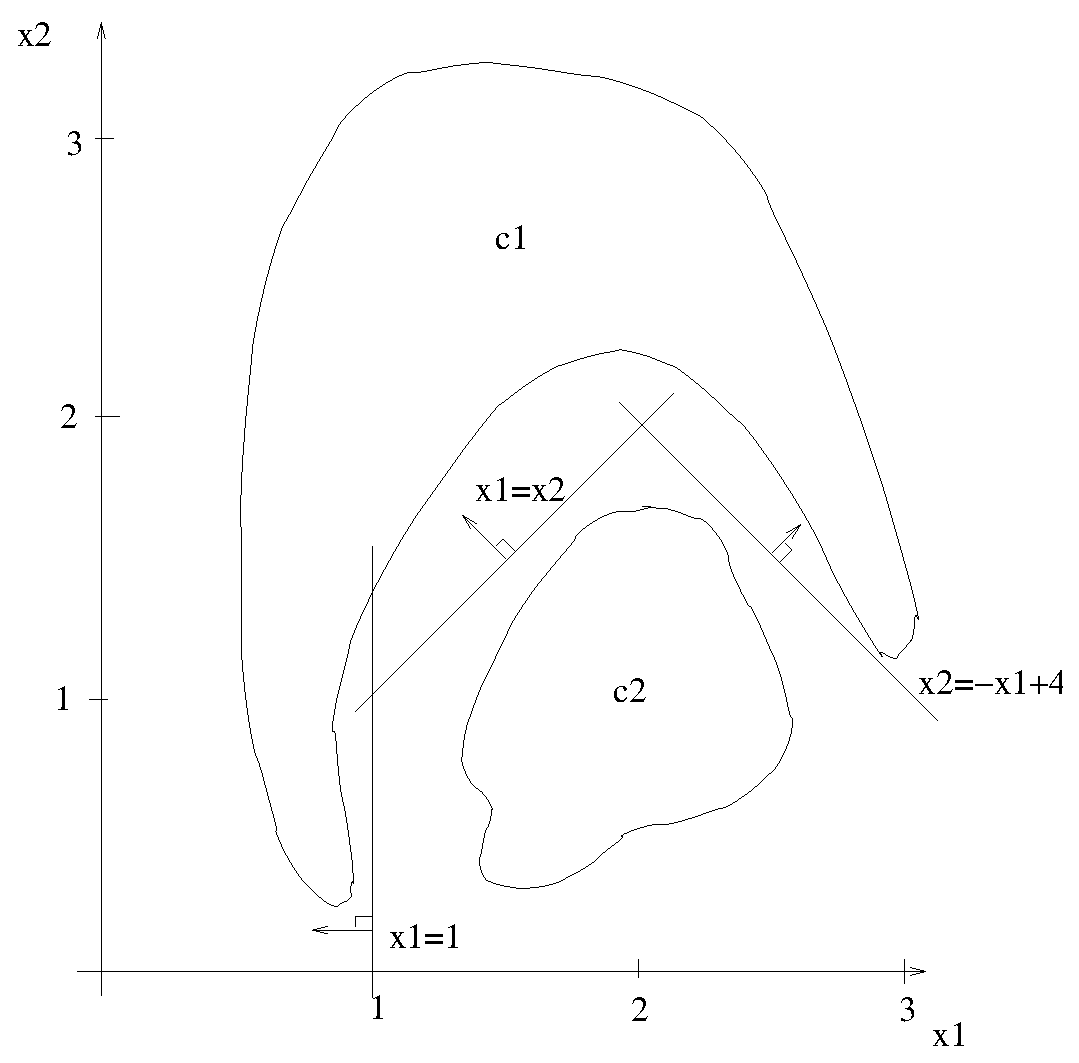
\includegraphics[scale=0.35]{e61}
    \end{center}

    The classification task can be solved using three linear classifiers
    such that $\vect{w}_i^T\vect{x}=0$ gives the classification for each
    linear classifier.

    The network:
    \begin{center}
      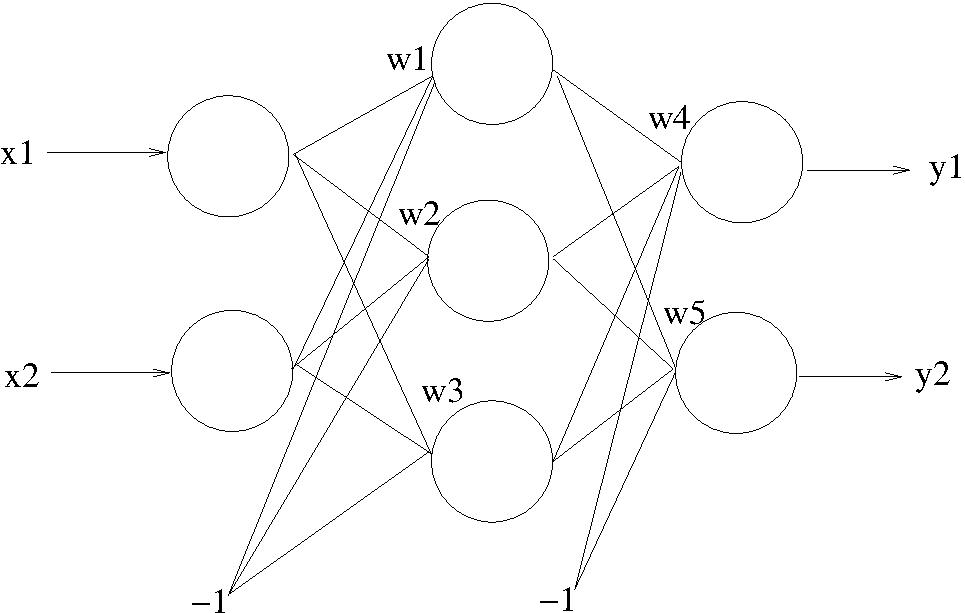
\includegraphics[scale=0.35]{e61-2}
    \end{center}
    % 
    The input to the network relates to the coordinate axis by
    $\mathbf{x} = \begin{pmatrix}x_1&x_2&-1\end{pmatrix}^T$ where the
    last component is the bias.  Each linear classifier uses the
    outputs of McCulloch-Pitts perceptrons which determined as
    follows:
    \begin{equation*}
      z_i=\left\{\begin{array}{l}
          1 \mbox{, if }\vect{w}_i^T\vect{x} > 0\\
          0 \mbox{, otherwise}
        \end{array}\right.
    \end{equation*}
    The parameters $\mathbf{w}_i$ for each hidden layer neuron can be
    derived from the above figure:
    \begin{equation*}
      \left.
        \begin{array}{lcrcl}
          i=1:\, \mathbf{x}_1<1& \Rightarrow
          & \begin{pmatrix}-1&0&-1\end{pmatrix}\mathbf{x}>0 &
          \Rightarrow &
          \vect{w}_1=\begin{pmatrix}-1&0&-1\end{pmatrix}^T
          \\
          i=2:\, \mathbf{x}_2>\mathbf{x}_1&
          \Rightarrow
          & \begin{pmatrix}-1&1&0\end{pmatrix}\mathbf{x}>0 & \Rightarrow &
          \vect{w}_2=\begin{pmatrix}-1&1&0\end{pmatrix}^T
          \\
          i=3:\, \mathbf{x}_2>-\mathbf{x}_1+4 &
          \Rightarrow
          & \begin{pmatrix}1&1&4\end{pmatrix}\mathbf{x}>0 &
          \Rightarrow & \vect{w}_3
          = \begin{pmatrix}1&1&4\end{pmatrix}^T 
        \end{array}\right\}\mbox{hidden layer}
    \end{equation*}
    

    Let $z_i \in\{0,1\}$ be the output of the $i$:th hidden layer
    neuron and
    $\vect{z}=\begin{pmatrix}z_1&z_2&z_3&-1\end{pmatrix})^T$.  Again,
    McCulloch-Pitts perceptrons are used and the weights of the output
    layer neurons, $\vect{w}_4$ and $\vect{w}_5$ are set so that
    \begin{equation*}
      \begin{cases}
        \vect{w}_4^T\vect{z} > 0, & \text{if } z_1=1 \text{ or } z_2=1
        \text{ or } z_3=1,
        \\
        \vect{w}_4^T\vect{z} \leq 0, & \text{otherwise}
      \end{cases}
    \end{equation*}
    and the opposite classification with $\vect{w}_4=-\vect{w}_5$.
    One feasible solution is
    $\vect{w}_4=\begin{pmatrix}1&1&1&\frac{1}{2}\end{pmatrix}^T$. However,
    the above problem has infinitely many solutions.
    \begin{enumerate}
    \item The minimum amount of neurons in the hidden layer is two as
      the classes can be separated with two lines.
    \item There is no upper limit for the number of hidden layer
      neurons. However, the network might overlearn the training set
      and lose its generalization capability. When the number of
      hidden layer neurons is increased, the boundary between the
      classes can be estimated more precisely.

    % \item Based on the universal approximation theorem we could state
    %   that the claim is true (or maybe it is just approximately
    %   true?).  However, let us provide a constructive proof which is
    %   more interesting and gives a method to find such a solution.

    %   One layer may not be sufficient in a complex case because the
    %   outputs of the hidden layer may not be linearly separable into
    %   classes.  Proof?

    %   Idea: Form the class as a collection of convex sets.  The first
    %   layer hidden determines whether the points are in the
    %   half-spaces (neuron per half-space).  The second hidden layer
    %   determines whether they are inside the convex sets (neuron per
    %   convex set).  The output layer determines whether they are
    %   inside at least one convex set (one neuron).

    %   The following proof misses the second hidden layer. It should be
    %   added. But still the question is, could this be achieved with
    %   one hidden layer?

    %   Note that any complex class can be contained in a union of convex
    %   sets.  It is assumed that the classes are separable, that is, they
    %   do not intersect, thus these convex sets may chosen such that they
    %   contain points only from one class and no points from other
    %   classes.
      
    %   A convex set can be constructed as an intersection of
    %   half-spaces.  These half-spaces are defined by hyperplanes which
    %   in turn correspond to neurons in the hidden layer (the weight
    %   vector of a neuron defines a hyperplane).  Thus, a collection of
    %   neurons can be used to represent one convex set: if the input
    %   vector is in the convex set, all the corresponding neurons
    %   should give output 1.  Thus, for one collection of $N$ neurons
    %   corresponding to one convex set, the input vector belongs to
    %   that convex set if
    %   \begin{equation}
    %     \sum^N_{i=1} z_i = N \quad \Rightarrow \quad
    %     \frac{1}{N}\sum^N_{i=1} z_i = 1, \label{eq:collection}
    %   \end{equation}
    %   which gives the following condition on the output layer:
    %   \begin{equation*}
    %     \frac{1}{N} \sum^N_{i=1} z_i > 1 - \epsilon,
    %   \end{equation*}
    %   where $\epsilon>0$ is a sufficiently small positive constant.  A
    %   sufficiently small value is $\epsilon<\frac{1}{N}$.

    %   % Now, the point belongs to the
    %   % class if it belongs to any of these convex sets.
    %   To obtain more convex sets, the hidden layer may contain several
    %   separate collections of neurons.  If for at least one of these
    %   neuron collections all the neurons output 1, then the input
    %   vector belongs to the class.  If the class is represented by $M$
    %   convex sets and the corresponding neuron collections are
    %   $A_1,\ldots,A_M$, it is sufficient that at least one collection
    %   satisfies \eqref{eq:collection}.  Thus, we have
    %   \begin{equation*}
    %     \sum_{j=1}^M \frac{1}{|A_j|} \sum_{z \in A_j} z > 1
    %     - \epsilon,
    %   \end{equation*}
    %   where $|A_j|$ is the number of neurons in the collection $A_j$
    %   and $\epsilon$ is chosen such that $\epsilon<\min_k
    %   \frac{1}{|A_k|+1}$.  This gives the weights and the bias term on
    %   the output layer.
      
    %   This proof showed how to select the hyperplanes, that is, the
    %   weights on the hidden layer.  The purpose of the hidden layer is
    %   to form convex sets that cover one class.  The proof also showed
    %   how to select the weights on the output layer in order to output
    %   $1$ if the input vector does belong to the class, that is, to
    %   any of the convex sets defined by the hidden layer.

    %   Although the classification can be performed using only one
    %   layer, the total number of neurons can sometimes be reduced if
    %   one uses several layers.  Thus, it is not necessarily a good
    %   idea to use only one layer although it is theoretically enough
    %   to give the correct classification.


    \end{enumerate}

  \end{solution}
  
\item The function
  \[
  t(x) = x^2, \hspace{3mm} x \in \left[ 1, 2 \right]
  \]
  is approximated with a neural network. The activation functions of all
  the neurons are linear functions of the input signals and a constant
  bias term. The number of neurons and the network architecture can be
  chosen freely. The approximation performance of the network is
  measured with the following error function:
  \[
  \mathcal{E} = \int_{1}^2 \left[ t({\bf x})-y({\bf x}) \right]^2 d{\bf x}
  \]
  where $\vect{x}$ is the input vector of the network and $y(\vect{x})$ is the
  corresponding response.
  \begin{itemize}
  \item[(a)] Construct a single-layer network which minimizes the error function.
  \item[(b)] Does the approximation performance of the network improve if
    additional hidden layers are included?
  \end{itemize}

  \begin{solution}

    (a) Output of a single-layer network is

    \begin{equation*}
      y(x)=Wx+\theta
    \end{equation*}
    and the approximation performance measure is
    \begin{align*}
      \mathcal{E}&=\int_1^2(t(x)-y(x))^2 dx
      \\
      &= \int_1^2 (x^2-Wx-\theta)^2dx
      \\
      &=\int_1^2 (x^4+\theta^2 +W^2x^2-2Wx^3+2W\theta x-2\theta x^2)dx
      \\
      &=\Big/^2_{\mspace{-11.0mu} 1} \frac{x^5}{5}
      +\theta^2x+\frac{W^2x^3}{3}-\frac{Wx^4}{2}+W\theta
      x^2-\frac{2}{3}\theta x^3
      \\
      &=\frac{31}{5}+\theta^2
      +\frac{7}{3}W^2-\frac{15}{2}W+3W\theta-\frac{14}{3}\theta
    \end{align*}

    Let us find $W$ and $\theta$ which minimize $\mathcal{E}$:
    \begin{align*}
      &
      \begin{array}{l}
        \begin{cases}
          \frac{\partial\mathcal{E}}{\partial
            W}=\frac{14}{3}W-\frac{15}{2}+3\theta = 0 & | \cdot 2
          \\
          \frac{\partial\mathcal{E}}{\partial
            \theta}=2\theta+3W -\frac{14}{3} = 0 & | \cdot (-3)
        \end{cases}
        \\
        \hline
        (\frac{28}{3}-9)W - 15 + 14 = 0 \quad \Rightarrow \quad W^*=3
      \end{array}
      \\
      \Rightarrow &
      \begin{cases}
        W^* = 3
        \\
        2\theta+3\cdot 3 -\frac{14}{3} = 0 \quad \Rightarrow \quad \theta^* =
        -2\frac{1}{6}
      \end{cases}
    \end{align*}

    As $\left.\begin{pmatrix} \frac{\partial^2\mathcal{E}}{\partial W^2} &
        \frac{\partial^2\mathcal{E}}{\partial W \partial\theta}\\
        \frac{\partial^2\mathcal{E}}{\partial W \partial\theta} &
        \frac{\partial^2\mathcal{E}}{\partial\theta^2}
      \end{pmatrix}\right|_{\begin{array}{l}\scriptstyle  W=W^*\\\theta=\theta^*\end{array}}$
    is positive definite, $\mathcal{E}$ gets its minimum value when
    $W=W^*$ and $\theta=\theta^*$.

    \vspace{0.5cm}
    (b) No because $y(x)=\sum_z w_{1z}^{(n)}\left(\sum_y
      w_{zy}^{(n-1)}\left(\dotsm \sum_a w_{a1}^{(1)}x\right)\dotsm\right) = Wx$. See
    exercise 1, problem 4.

  \end{solution}

% \item I implemented the experiment in Haykin section 3.11 in
%   \texttt{ex04_03.m} but a) it might not be correct and b) I don't see
%   the point of that experiment.


\end{enumerate}
\end{document}             % End of document.
